\scanpage{28}
% archive sheet number: 27
% L1–4
\uline{Facettes} d'un ens convexe $C$ (dans vectoriel réel) :
partie \deleted{\unsure{convexe}} \deleted{\unsure{$C'$}} non vide $F$ de $C$ telle que
\deleted{$x\in F$, $y\in C-F$ implique que $x$ \inserted{ou $y$} est une extrémité de $C\cap D_{xy}$ [où $D_{x,y}$ est
la droite qui joint $x$ et $y$, i.e. l'ens des $tx+(1-t)y$ $(t\in\mathbb R)$]}
\deleted{On \unsure{aura|a donc|convexe} :}

% L5–9
pour $x\in F$, $y\in C-\{x\}$, \deleted{\unsure{et}} \inserted{on a $y\in F$ \unsure{ss|ssi|si}} \deleted{si} $x$ \inserted{ni $y$} n'est \deleted{\unsure{pas}} une
extrémité de $C\cap D_{xy}$ (i.e. s'il exist $x',y'\in C\cap D_{xy}$ tel que
$x,y$ \deleted{sont} \inserted{soient} entre $x'$ et $y'$
\figure{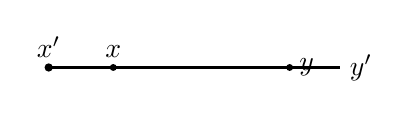
\begin{tikzpicture}[x=1cm,y=1cm]
\draw[thick](0,0)--(3.7,0);
\fill (0,0) circle (1.5pt) node[above]{$x'$};
\fill (.82,0) circle (1.25pt) node[above]{$x$};
\fill (3.06,0) circle (1.25pt) node[right]{$y$};
\node[right] at (3.7,0){$y'$};
\end{tikzpicture}}
) alors $y\in F$. On peut l'exprimer aussi en disant que
tt intervalle ouvert $\subset C$ qui rencontre $F$ est contenu ds $F$.

% L10–13
\uline{Prop} Toute facette de $C$ est convexe, \inserted{(non vide)}. $C$ est \deleted{\unsure{l'}}réunion disjointe de ses facettes

Considérons la relation dans $C$
\[
 R(x,y):\quad(x=y)\ \text{\uline{ou}}\ (x\text{ ni }y\text{ n'est extrémité de }C\cap D_{xy})
\]
\inserted{i.e. $x,y\in$ un intervalle ouvert $\subset C$}
\figure{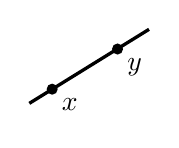
\begin{tikzpicture}[x=1cm,y=1cm]
\draw[very thick](0,0)--(1.52,.94);
\fill (.29,.18) circle (2pt) node[below right]{$x$};
\fill (1.12,.69) circle (2pt) node[below right]{$y$};
\end{tikzpicture}}

% L14–18
c'est une relation \deleted{\unsure{au moins}} d'équivalence : \unsure{réfl.} \inserted{\unsure{sym.}} évident ;
transitivité facile. Il est \unsure{clair|découle} aussi que
$\forall x\in C$, la classe de $x$ suivant
$R$ est l'unique facette qui contient $x$.

\figure{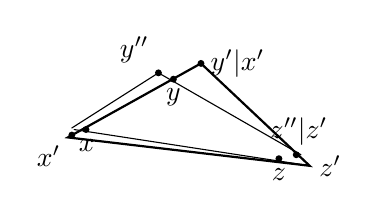
\begin{tikzpicture}[x=1cm,y=1cm,line cap=round]
\draw (.05,.12)--(1.15,.82)--(2.96,-.22);
\draw[thick](0,0)--(1.69,.94)--(3.07,-.36)--cycle;
\draw (.08,.10)--(3.07,-.36);
\foreach \x/\y in {.05/.03,.23/.10,1.15/.82,1.34/.74,1.69/.94,2.68/-.27,2.90/-.22}{\fill (\x,\y) circle(1.25pt);}
\node[below left] at (.03,.02){$x'$};
\node[below] at (.24,.1){$x$};
\node[above left] at (1.15,.82){$y''$};
\node[below] at (1.34,.74){$y$};
\node[right] at (1.69,.94){$\unsure{y'|x'}$};
\node[below] at (2.68,-.27){$z$};
\node[above] at (2.93,-.23){$\unsure{z''|z'}$};
\node[right] at (3.07,-.36){$z'$};
\end{tikzpicture}}

% L19–25
\uline{Prop} Soit $C$ un \uline{polyèdre} convexe (i.e. un ens
convexe qui est réunion finie d'enveloppes
\deleted{\unsure{f}} convexes de parties finies de l'espace affine
$E$)
% slanted
\margin{ou encore : int. \uline{finie} de demi-espaces fermés\ldots}
alors : \textcircled{1} l'ens des facettes est \uline{fini}. \textcircled{2} $\exists$ unique
facette maximale $\unsure{P|\mathcal P|\Phi}$, qui est aussi l'int de $C$ dans l'espace
affine engendré par $C$.

\textcircled{3} Pour tte facette $F$, $\overline F$ est une réunion de
facettes \deleted{\unsure{et on a} $\overline F\unsure{=|\supset} F'$ \unsure{(cf formule)|($F,F'$ facettes)} \unsure{ssi} $F=F'$}
\inserted{et, $F$ est l'unique facette $\subset\overline F$ de dimension max ($=\dim\overline F$)}

% L26–28 and lower left margin
\textcircled{4} et si celle ci est $d$, $\exists$ facette $\subset\overline F$ de dim $d-1$

% slanted
\margin{\textcircled{5} $C$ est l'env. convexe de la réunion \deleted{\unsure{des}} des facettes minimales ($=$ les pts extrémaux)}
% slanted
\margin{\textcircled{\unsure{6}} \deleted{\unsure{le}} \uline{bar.} de l'ens des pts extr. \unsure{ou des} facettes \unsure{minimales} \unsure{est au centre|est un centre|caractérise}}
\uline{Cor} Si $F,F'$ sont des facettes, $\overline F=\overline{F'}\Rightarrow F=F'$

Relation d'ordre entre facettes
